\section{JSON}
\label{sec:json}

JavaScript Object Notation (JSON) ist eine Syntax zum Definieren von Datenaustauschformaten. Diese ist textbasiert, simpel, und vor allem sprachunabhängig, was sie zu einem sehr verbreiteten Format für den Austausch strukturierter Daten im Internet macht. JSON wird von 99,71 \% der Browser unterstützt (gewichtet nach Marktanteil) [\cite{jsonBrowser}].\\
Ursprünglich wurde JSON aus der Syntax für Objektnotationen von der Programmiersprache ECMAScript (weithin bekannt als JavaScript) abgeleitet, doch der Standard für JSON [\cite{json}] hat dessen Strukturierungsregeln abstrahiert, sodass nun die meisten Sprachen in der Lage sind, JSON zu parsen.\\
Der Satz dieser Regeln besteht lediglich aus den rekursiven Definitionen von \verb|object|, \verb|array|, \verb|value|, \verb|string|, \verb|number|, und \verb|whitespace|. In Grafik \ref{fig:JSON} ist beispielhaft die Definition eines Objektes dargestellt.
%
\begin{figure}[htbp]
	\centering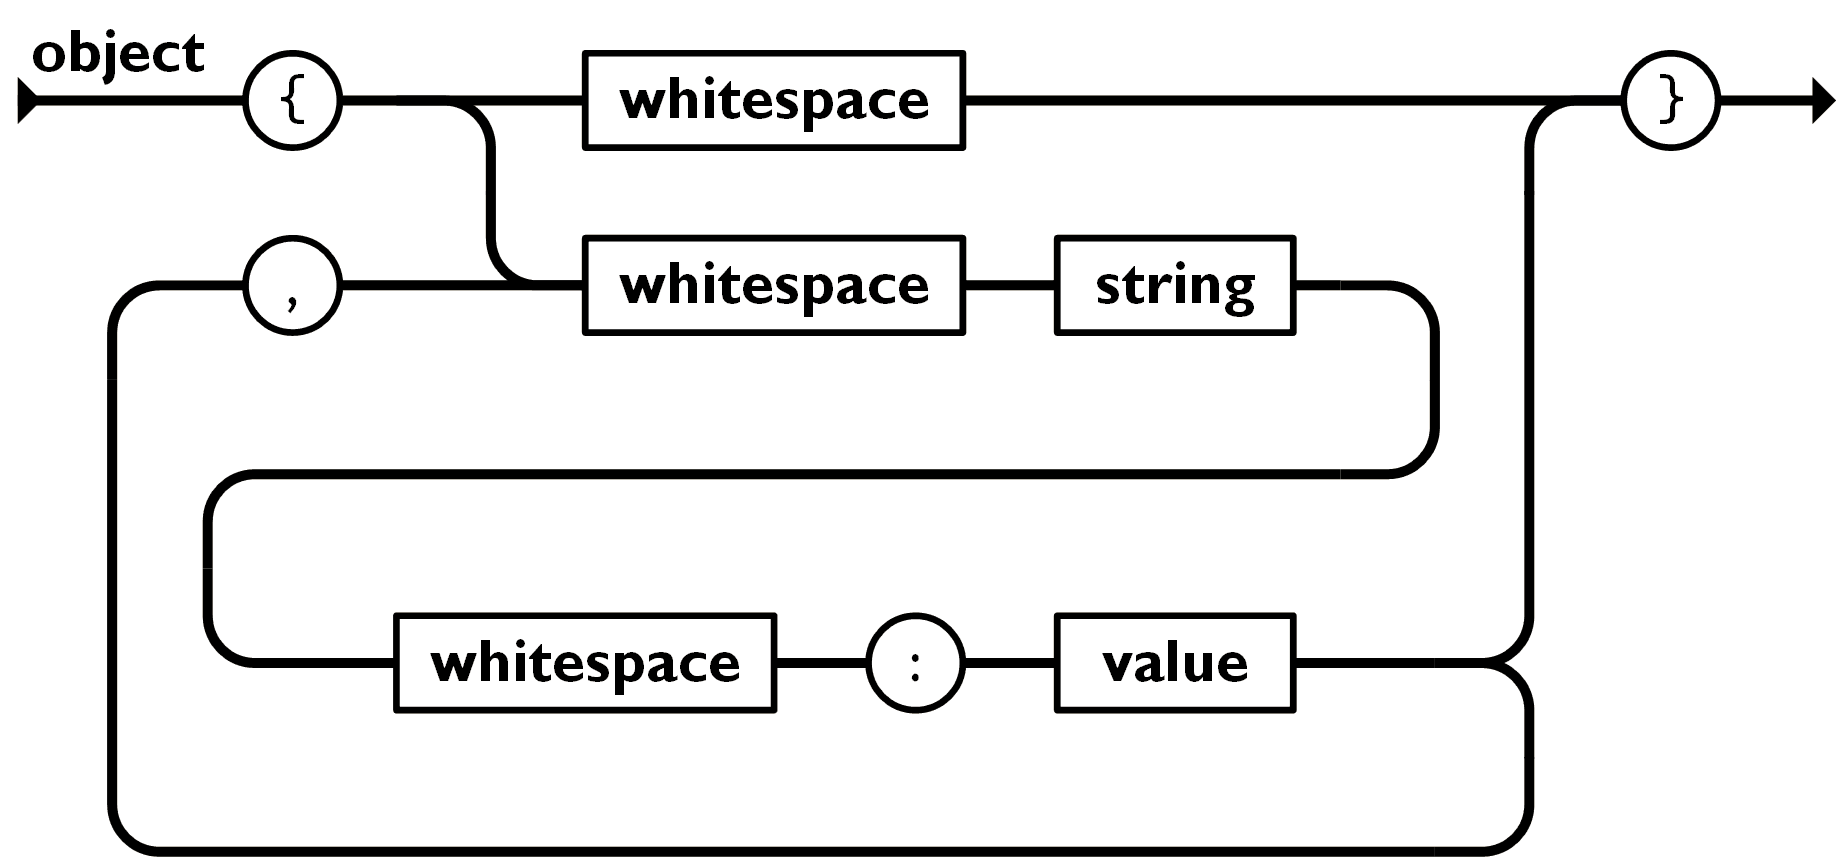
\includegraphics[width=0.7\textwidth]{images/03/JSON.png}
    \caption{Definition eines Objektes in JSON [\cite{jsonDefinition}]}
    \label{fig:JSON}
\end{figure}

Ein wesentlicher Nachteil von JSON als Format für die Datenübertragung im Internet ist jedoch, dass JSON aufgrund seiner Struktur nicht streambar ist. Dies ist vordergründig im Kontext des Internets ein Problem, denn auch mit modernen Upload-/Downloadgeschwindigkeiten liegt der rechentechnische Engpass bei der Datenübertragung. Andere Datenformate wie XML können gestreamt werden, das heißt, sie können geparst und verarbeitet werden, noch während sie übertragen werden. JSON dagegen muss vollständig übertragen werden, bevor es von einem Programm verarbeitet werden kann. Dies ist jedoch in der Regel nur bei Echtzeitsystemen oder sehr großen übertragenen Datenmengen relevant.
